\documentclass{rapport}
\title{Rapport} %Titre du fichier
\usepackage{amsmath}
\usepackage{longtable}
\usepackage{listings}

\begin{document}

%----------- Informations du rapport ---------

\logo{logos/UMONS.png}
\unif{UMONS}
\titre{Projet d'optimisation linéaire} %Titre du fichier .pdf
\cours{Optimisation linéaire} %Nom du cours
\sujet{Récupération d’une image floutée (deblurring)}

\enseignant{Nicolas \textsc{Gillis}} %Nom de l'enseignant

\eleves{Nicolas \textsc{Gatta} \\
		Arnaud \textsc{Schellekens}} %Nom des élèves

%----------- Initialisation -------------------
        
\fairemarges %Afficher les marges
\fairepagedegarde %Créer la page de garde
\tabledematieres %Créer la table de matières

%------------ Corps du rapport ----------------


\section{Introduction} 

L’objectif de ce projet est l’étude du problème de minimisation $\min_{0 \le x \le 1} \| Ax-\tilde{x} \|_1 + \lambda \| x \|_1$ qui permettra de reconstruire une image non floutée et non bruitée à partir d’une image floutée et bruitée.

\section{Question 1: Modélisation du problème}
Il faut écrire le problème ci-dessus sous forme d’un problème d’optimisation linéaire: 
\begin{equation}
    \min_{0 \le x \le 1} \| Ax-\Tilde{x} \|_1 + \lambda \| x \|_1
\end{equation}
Nous savons que la norme 1 d’un vecteur est la somme des valeurs absolues de ses composantes, on applique cela dans la formule (1) ce qui nous donne:
\begin{equation}
    \min_{0 \le x \le 1} \sum_{i=1}^n |a_i x-\Tilde{x}_i | + \lambda |x_i|
\end{equation}
Grâce au $a_i$ la n-ième ligne de A, $x_i$ la n-ième ligne de x et n le nombre de lignes de A et $\Tilde{x}$. En effet, ces matrices doivent avoir le même nombre de lignes et de colonnes dans le cas d’une addition/soustraction et doivent avoir le même nombre de lignes pour une multiplication pour que celles-ci puissent se produire. Enfin, en traitant les valeurs absolues, on obtient :
\begin{equation}
    \begin{aligned}
        \min_{xi} \quad&\sum_{i=1}^n t_i + \lambda|x_i|\\
        \textrm{t.q.} \quad 
            &t_i\geq a_ix_i-\Tilde{x_i}\\
            &t_i\geq -a_ix_i+\Tilde{x_i}\\
            &x_i\geq 0\\
            &x_i\leq1\
    \end{aligned}
\end{equation}


\section{Question 2: Forme standard}

Nous devons écrire le problème d’optimisation linéaire formulé à la question 1 sous forme standard.
\begin{equation}
    \begin{aligned}
        \min_{xi} \quad&\sum_{i=1}^n t_i + \lambda x_i\\
        \textrm{t.q.} \quad 
            &t_i -s_1= a_i x-\Tilde{x}_i\\
            &t_i -s_2= -a_i x+\Tilde{x}_i\\
            &x_i + s_3 = 1\\
            &x_i \ge 0\\
            &s_1, s_2, s_3 \ge 0
    \end{aligned}
\end{equation}

\section{Question 3: Déflouter une image}

Pour déflouter une image, on utilise comme demander dans la question la fonction \textbf{\textit{glpk}} de Octave. Cette fonction va nous permettre de résoudre le problème d’optimisation linéaire suivant :
\begin{equation}
    \begin{aligned}
        \min_{0 \le x \le 1} \quad&\sum_{i=1}^n t_i + \lambda \tilde{x}_i\\
        \textrm{t.q.} \quad & -t_i+a_i x \le \tilde{x}_i\\
        & -t_i-a_i x \le - \tilde{x}_i\\
    \end{aligned}
\end{equation}
Pour faire fonctionner la fonction de \textbf{\textit{glpk}}, il a fallu remplacer les deux contraintes $x\ge 0$ et $x \le 1$ par des matrices d'une colonne et de n lignes (correspondant à la taille de $\Tilde{x}$) remplies de 0 pour {\bf lb} (borne inférieure) et remplies de 1 pour {\bf ub} (borne supérieure).\\\\
En plus de cela, il a fallu créer une nouvelle variable contenant les types de contraintes utilisés pour chaque ligne. Vu que nous avons pris le temps de convertir toutes les contraintes « $\le$ », la variable {\bf cty} (type de contrainte) va être remplie de « U » correspondant aux contraintes avec des bornes supérieures.\\\\
Enfin, les n derniers éléments de la solution renvoyés par la fonction \textbf{\textit{glpk}} vont être sélectionnés pour afficher l’image défloutée et débruitée, car les n premiers éléments correspondent aux $t_i$ et les n derniers correspondent aux $x_i$
\section{Question 4: Le polyèdre}
Il faut déterminer si la solution obtenue est un sommet du polyèdre c'est-à-dire si la solution est une solution admissible de base. La solution $x$ est une solution admissible de base s’il y a n contraintes actives et linéairement indépendantes en $x$. Comme vu en cours, la solution du problème est un sommet du polyèdre. Cette réponse peut être obtenue via l’algorithme \textbf{estSommet} fonctionnant de la manière suivante :\\
	
\begin{itemize}
    \item [\textbullet]Il crée une matrice vide ({\bf actives})  qui regroupera, les contraintes actives.
    \item [\textbullet]Pour chaque contrainte, il vérifie si elle est active en $x$ et si elle l’est, il la rajoute dans la matrice.
    \item [\textbullet]Il calcule le rang de la matrice qui est le nombre de contraintes linéairement indépendantes. On a alors le nombre de contraintes actives et linéairement indépendantes. 
    \item [\textbullet]On a besoin de trouver $2n-m$ contraintes actives et linéairement indépendantes. Nous cherchons ces contraintes dans les contraintes de positivité et de $x_i \le 1$.
    \item [\textbullet]Si le nombre de contraintes actives et linéairement indépendantes est plus grand ou égal à $2n$ alors la solution est donc un sommet du polyèdre.
\end{itemize}
\newpage
\section{Question 5: Sensibilité de la solution}
Pour cette question, il faut étudier la sensibilité de la solution en fonction de la valeur de $\lambda$ pour les images Example0.mat et Example1.mat. Les valeurs des erreurs relatives en fonction de la valeur de $\lambda$ sont reprises dans les tableaux ci-dessous: \\\\
Pour « Example0.mat », on remarque que la valeur de $\lambda$ qui convient le mieux sont les valeurs égales ou plus petites que 0 alors que la valeur qui convient le moins est 1:
\begin{longtable}{|c|c|} 
    \hline
    Valeurs de lambda & Erreur relative de reconstruction \endhead
    \hline
    1&82.5734 \%\\ 
    0&1.23e-12 \%\\ 
    1e-1&3.81e-12 \%\\ 
    1e-2&9.75e-12 \%\\ 
    1e-3&2.24e-12 \%\\ 
    1e-4&1.31e-12 \%\\ 
    1e-5&1.23e-12 \%\\ 
    1e-6&1.23e-12 \%\\ 
    1e-7&1.23e-12 \%\\ 
    1e-8&1.23e-12 \%\\ 
    1e-9&1.23e-12 \%\\ 
    1e-10&1.23e-12 \%\\ 
    \hline
\end{longtable}
Pour « Example1.mat », il est malheureusement impossible d'utiliser la méthode vu que le fichier ne possède aucune variable xtrue étant la variable permettant de recréer l'image de base et ainsi pouvoir la comparer au résultat obtenu grâce à l'algorithme. \\
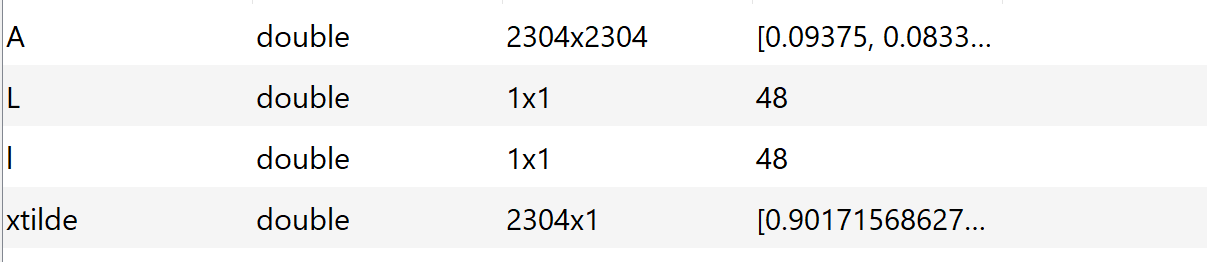
\includegraphics[width=\textwidth]{logos/image2.png}
\newpage
\section{Annexe}
\UseRawInputEncoding

\subsubsection{deblurr}
\lstinputlisting{Code/deblurr.m}

\newpage
\subsubsection{main}
\lstinputlisting{Code/MainFile.m}

\newpage
\subsubsection{testLambda}
\lstinputlisting{Code/testLambda.m}

\newpage
\subsubsection{estSommet}
\lstinputlisting{Code/estSommet.m}
\end{document}
